\subsection{Ricerca degli utenti}
La ricerca degli utenti è stata fatta in maniera completamente telematica per via delle misure restrittive attualmente in vigore nel territorio nazionale.\\
Non avendo la possibilità di contattare direttamente un sufficiente numero di giornalisti abbiamo proceduto come illustrato di seguito.

\subsubsection{Intervista telefonica}
Avevamo a disposizione un solo contatto di una giornalista di \textit{SkyTG24}, Roberta, ed è stata quindi contattata telefonicamente per un'intervista.
Di seguito vengono riportate le domande poste e, riassunte, le risposte ricevute\footnote{L'audio integrale dell'intervista e gli spezzoni con le risposte sono presenti tra i file consegnati per il progetto.}:
\begin{enumerate}
    \item \textbf{Domanda}: Quanto spesso usi la dashboard del DPC?\\\textbf{Risposta}: Quotidianamente, perché è necessaria al fine di tenere d'occhio l'andamento della pandemia. Viene costantemente aggiornata la pagina per verificare la presenza di nuovi dati.
    \item \textbf{Domanda}: Cosa ne pensi delle funzionalità e dell’impatto grafico della dashboard?\\\textbf{Risposta}: La dashboard è abbastanza intuitiva e funziona abbastanza bene, ma graficamente è poco accattivante, data la pervasione del colore nero.
    \item \textbf{Domanda}: Cosa ne pensi dei dati mostrati (parte 1)?\\\textbf{Risposta}: Sono presenti solo dati assoluti e sarebbe invece interessante offrire dati rapportati (per esempio: $tasso\; di\; positivit\grave{a} = \frac{tamponi\; positivi}{tamponi\; effettuati}$, in un giorno)
    \item \textbf{Domanda}: Come analizzate voi in SkyTG24 i dati della pandemia (parte 1)?\\\textbf{Risposta}: Si è consolidato un processo di business che fornisce una lista di valori di metriche automaticamente calcolate (come avverrebbe in un foglio di calcolo) a partire da dati ricevuti da organizzazioni esterne (per esempio dal DPC, dall'Istituto Superiore di Sanità (ISS)).
    \item \textbf{Domanda}: Cosa ne pensi dei dati mostrati (parte 2)?\\\textbf{Risposta}: I dati mostrati, con l'avanzare delle settimane e dei mesi, diventano sempre più grandi e hanno sempre più meno senso, se presi in assoluto. Dati come il numero degli attuali positivi o dei guariti, purtroppo, non aiutano molto nella comprensione dell'andamento. Dati come gli attuali ricoveri in terapia intensiva e ospedalizzazioni non ci sono (a onor del vero ci sarebbero sia quelli a livello nazionale, ma non vengono mostrati, sia quelli a livello regionale, ma sono nascosti). Sarebbe utile, inoltre, avere una correlazione dei dati del DPC con quelli dell'ISS, che raccoglie informazioni quali l'età mediana e la distribuzioni rispetto alla popolazione.
    \item \textbf{Domanda}: Cosa ne pensi dei grafici e della mappa mostrati?\\\textbf{Risposta}: Sono grafici poco spiegati, che presentano delle curve di andamento ma non si capisce come interpretarle. Inoltre, la mappa dell'Italia, che occupa la maggior parte della dashboard non ha un funzionamento chiaro.
    \item \textbf{Domanda}: Come analizzate voi in SkyTG24 i dati della pandemia (parte 2)?\\\textbf{Risposta}: Vengono utilizzati i bollettini quotidiani del DPC e informazioni provenienti da un sistema realizzato da dei \textit{Data journalist} che automaticamente invia una mail alla loro redazione.
    \item \textbf{Domanda}: Sarebbe comoda una dashboard unica?\\\textbf{Risposta}: Ovviamente sì. L'importante è che i dati siano comprensibili, che siano spiegati; i giornalisti ormai sanno abbastanza destreggiarsi fra le varie terminologie e interpretazioni dei dati ma ai cittadini questo manca. Tutti dovrebbero poter comprendere i dati presentati dalla dashboard.
    \item \textbf{Domanda}: La difficoltà nella lettura dei dati inficia la qualità degli articoli prodotti?\\\textbf{Risposta}: Sì e anche le istituzioni dovrebbero fornire gli strumenti per analizzarli con più facilità.
    \item \textbf{Domanda}: La giornalista ci informa a riguardo di un'altra fonte di informazione.\\\textbf{Risposta}: Esiste un'altra fonte, che presenta dati e quindi dei cruscotti sull'andamento della pandemia: è l'Agenzia Nazionale per i Servizi Sanitari Regionali (AGENAS). Fornisce informazioni sullo stato delle terapie intensive, ospedali e pronti soccorsi nelle varie regioni e a livello nazionale. Perché questa fonte preziosa non è pubblicizzata a dovere? Perché questi dati non sono integrati nella dashboard del DPC?
    \item \textbf{Domanda}: Sarebbe interessante la possibilità di fornire un confronto tra nazioni, regioni, province e i loro indicatori?\\\textbf{Risposta}: Ha poco senso fornire il confronto fra nazioni se la dashboard è sull'Italia. È invece utile fornire il confronto tra regioni (tra province meno, in quanto le province non hanno colori - rosso, arancione, giallo - a differenza delle regioni), seppur potrebbe esserci mancanza di dati in caso le istituzioni non li forniscano.
    \item \textbf{Domanda}: Sarebbe interessante un confronto rispetto al numero di tamponi effettuati?\\\textbf{Risposta}: Potrebbe essere utile ma c'è da porre attenzione su un confronto di questo tipo: le regioni potrebbero contare fra i tamponi effettuati anche i tamponi rapidi, non solo quelli molecolari. Un confronto di questo tipo potrebbe essere fuorviante.
    \item \textbf{Domanda}: Sarebbe interessante un confronto rispetto al numero dei decessi?\\\textbf{Risposta}: Sì, ma correlati di altri dati su età, sesso, malattie pregresse e dove abitano.
\end{enumerate}

\subsubsection{Questionario online}
Anche riuscendo a reperire più contatti di giornalisti, non sarebbe stato possibile svolgere un'intervista telefonica cercando di riuscire a soddisfare le esigenze di tutti in un breve periodo temporale.\\
Abbiamo provveduto di conseguenza a realizzare un questionario online, attraverso \textit{Google Forms}.

\paragraph{La scelta delle domande}\mbox{}\\
In questo questionario sono stati posti i seguenti quesiti agli intervistati.
\begin{itemize}
    \item[1)] Indichi il suo livello di familiarità con l'utilizzo del computer e di Internet (una sola risposta):
    \begin{itemize}
        \item Principiante (Uso poche app sul telefono, navigo solamente sui siti che già conosco, uso pochi programmi al computer);
        \item Intermedio (ho una certa dimestichezza con la tecnologia, uso funzioni avanzate dello smartphone e svolgo diverse attività al computer);
        \item Esperto (ho familiarità con i dispositivi tecnologici, ne personalizzo l'uso in base alle mie esigenze).
    \end{itemize}
    \item[2)] Qual è la fonte principale da cui attinge dati sull'andamento dei dati relativi alla pandemia Covid-19 (una sola risposta)?
    \begin{itemize}
        \item Pubblicazioni di agenzie di stampa;
        \item Dashboard (qualsiasi);
        \item Bollettini della Protezione Civile;
        \item Altro... (campo di testo libero).
    \end{itemize}
\end{itemize}
In base al risultato di questa risposta, il questionario forniva all'utente una domanda 3 diversa: agli utenti che hanno risposto ``Dashboard (qualsiasi)" veniva presentata la successiva domanda \textit{3a)}, a tutti gli altri la domanda \textit{3b)}.
\begin{itemize}
    \item[3a)] Quali sono le dashboard che visita più spesso (più risposte possibili)?
    \begin{itemize}
        \item Protezione civile (Italia) (\href{http://arcg.is/C1unv}{http://arcg.is/C1unv});
        \item Istituto Superiore di Sanità (\href{https://www.epicentro.iss.it/coronavirus/sars-cov-2-dashboard}{https://www.epicentro.iss.it/coronavirus/sars-cov-2-dashboard});
        \item CSSE John Hopkins University (\href{https://bit.ly/2VBW7V6}{https://bit.ly/2VBW7V6});
        \item Lab24 (Il Sole 24 Ore) (\href{https://lab24.ilsole24ore.com/coronavirus/}{https://lab24.ilsole24ore.com/coronavirus/});
        \item World Health Organization (WHO) (\href{https://covid19.who.int/}{https://covid19.who.int/});
        \item Bing (\href{https://bing.com/covid/local/italy}{https://bing.com/covid/local/italy});
        \item Worldometer (\href{https://www.worldometers.info/coronavirus/?}{https://www.worldometers.info/coronavirus/?});
        \item Altro... (campo di testo libero).
    \end{itemize}
    \item[3b)] Ha indicato che le dashboard non sono la fonte principale tramite cui recupera i dati per i suoi articoli. Per quale/i motivo/i (più risposte possibili)?
    \begin{itemize}
        \item Non riesco ad interagirci;
        \item Sono troppo confusionarie;
        \item Riportano pressoché dati assoluti che non riesco a contestualizzare;
        \item Non conosco alcuna dashboard;
        \item Altro... (campo di testo libero).
    \end{itemize}
    \item[4)] Quanto tempo impiega per comprendere i dati sull'andamento della pandemia, prima di scriverci un articolo (una sola risposta)?
    \begin{itemize}
        \item Dai 5 ai 10 minuti;
        \item Dai 10 ai 15 minuti;
        \item Dai 15 ai 20 minuti;
        \item Dai 20 ai 25 minuti;
        \item Più di 25 minuti.
    \end{itemize} 
    \item[5)] Supponiamo esista una dashboard più chiara che le permetta, agevolmente, di contestualizzare ed interpretare i dati dell'andamento dei dati relativi alla pandemia Covid-19. Penserebbe di consultarla prima di scrivere i suoi articoli (una sola risposta)?
    \begin{itemize}
        \item Sì
        \item No
    \end{itemize}
    \item[6)] Quali informazioni (metriche, grafici, valori, ecc.) vorrebbe che la sua dashboard di riferimento le fornisse (più risposte possibili)?
    \begin{itemize}
        \item Contesto con cui rapportare i diversi valori (ad esempio, decessi ogni 100.000 abitanti, rapporto tamponi positivi/tamponi effettuati, ecc.);
        \item Saturazione terapie intensive;
        \item Eventuali ordinanze regionali;
        \item Elementi grafici interattivi in cui poter personalizzare la ricerca;
        \item Altro... (campo di testo libero).
    \end{itemize} 
    \item[7)] Sarebbe disposto a lasciarci un indirizzo mail a cui contattarla in caso avessimo bisogno di altre informazioni? Se sì, può scriverlo qui sotto, altrimenti può saltare la domanda (campo di testo libero).
\end{itemize}

\paragraph{Raccolta indirizzi e-mail per contattare i giornalisti}{}\mbox{}\\
Al fine di contattare quanti più giornalisti possibili, è stata raccolta una lista di indirizzi e-mail personali e redazioni, ricercandole all'interno delle sezioni \textit{Contatti} dei siti web dei giornali stessi, dai profili sui social, da conoscenze personali e da alcune newsletter ricevute.\\
La ricerca si è dovuta spostare necessariamente anche su \textit{LinkedIn}, dato che i contatti di alcuni giornalisti, specialmente di quelli di testate nazionali (per esempio di \textit{Open} o di \textit{Repubblica}), non erano altrimenti reperibili.\\
Una volta raccolto un numero sufficiente di contatti, è stata spedita la seguente mail (messaggio per quelli contattati su \textit{LinkedIn}) a tutti quanti loro:\\
\subfile{questionario-online/raccolta-indirizzi-mail-per-contattare-giornalisti/email}
Dopo aver spedito la mail la mattina del 07/12/2020, due giorni dopo avevamo ricevuto solo due risposte.
Essendo insufficienti per trarre conclusioni significative statisticamente, si è provveduto a creare una pagina su \textbf{Facebook} a nome del gruppo di progetto (la pagina è accessibile attraverso \href{https://www.facebook.com/XSparkUnibo}{questo link}).

\paragraph{Sponsorizzazione del questionario attraverso Facebook}\mbox{}\\
Dopo aver creato la pagina su \textit{Facebook}, dal nome \textit{X-Spark}, è stato pubblicato un post al fine di poterlo sponsorizzare e indirizzarlo a giornalisti italiani, rimandandoli al questionario creato.\\
Il contenuto del post è stato necessariamente più breve di quello della precedente mail, in quanto un testo della lunghezza simile non sarebbe stato letto da quasi nessuno.

\begin{figure}[!h] 
    \centering 
    
\includegraphics[width=0.4\columnwidth]{assets/images/ricerca-etnografica/post-facebook} 
    \caption{Post pubblicato attraverso la pagina \textit{Facebook} del gruppo.}
\end{figure}

Il post e il questionario sono stati sponsorizzati per 6 giorni, da mercoledì 09/12/2020 a lunedì 14/12/2020, avendo fissato un budget di \e{6}, da dividere in tre persone (non sapevamo il risultato della campagna di sponsorizzazione per cui siamo stati molto cauti con la spesa).\\
Il risultato finale è stato quello di raccogliere, oltre alle precedenti 2 risposte, altre 14, portando ad un totale di 16 risposte.\\
Gli strumenti di \textbf{Facebook} permettono di ottenere informazioni dettagliate su come è andata la sponsorizzazione, che riportiamo di seguito.

\begin{figure}[!h] 
    \centering 
    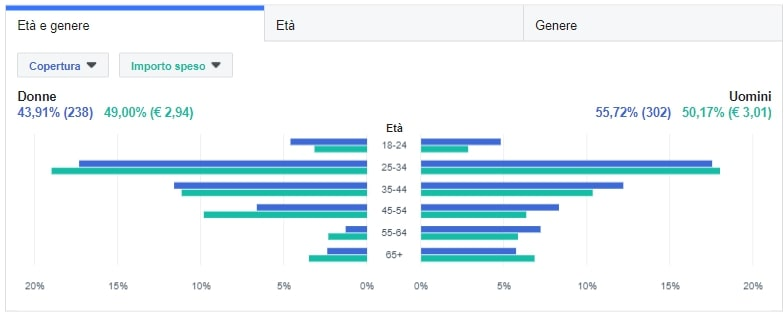
\includegraphics[width=0.9\columnwidth]{assets/images/ricerca-etnografica/post-facebook-statistiche-eta-genere} 
    \caption{Distribuzione dell'età e del genere degli intervistati.}
\end{figure}
Come si evince dal grafico, sono stati raggiunti in totale 542 giornalisti (auto-dichiaratisi\footnote{Per auto-dichiarati si intendono coloro che su \textit{Facebook} hanno impostato come professione ``Giornalista", ``Giornalista pubblicista" e simili. Non è possibile assicurarsi che ogni persona raggiunta sia effettivamente un giornalista, ma l'analisi delle risposte date, in particolare a quelle della domanda 7), portano a pensare che lo fossero tutti.} tali) uomini in misura maggiore (55,72\% degli uomini contro il 43,91\% delle donne), differenza accentuata soprattutto nelle fasce di età dai 55 anni in su.

\begin{figure}[!h]
    \centering
    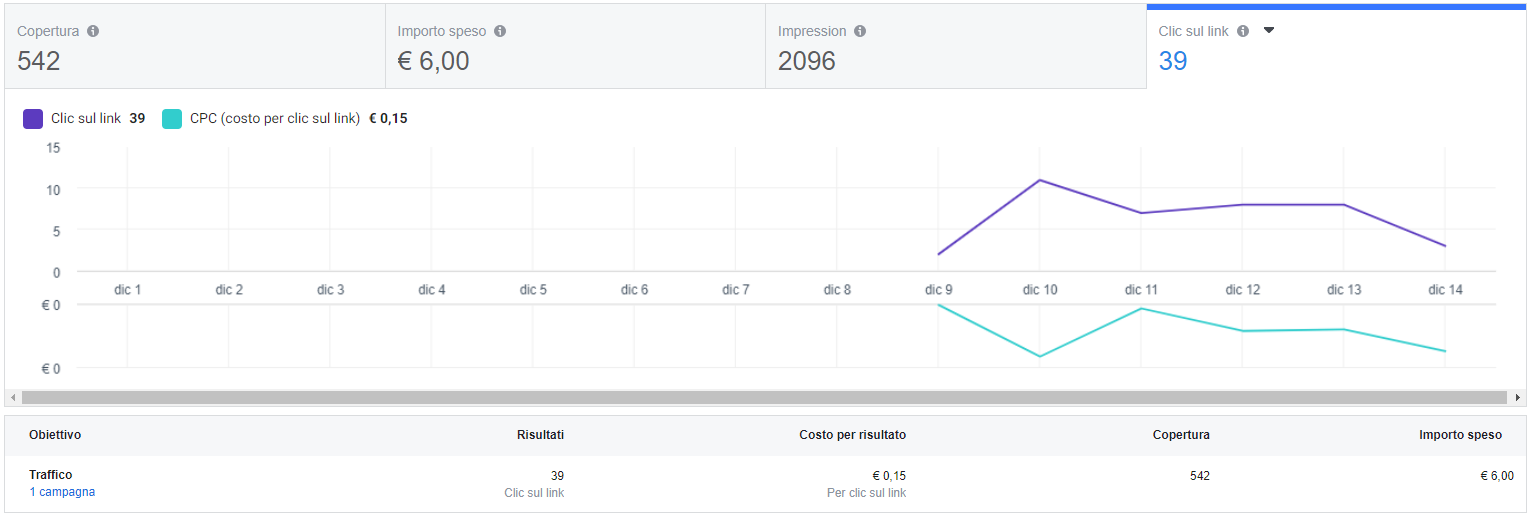
\includegraphics[width=0.9\columnwidth]{assets/images/ricerca-etnografica/post-facebook-statistiche-click}
    \caption{Distribuzione dei click nelle varie giornate.}
\end{figure}
Purtroppo, nonostante i 542 utenti di \textit{Facebook} raggiunti, solamente un totale di 39 utenti hanno deciso di cliccare sul questionario, che equivale al 7,1\% di loro. Molto pochi, se viene poi considerato che solo 14 di loro hanno deciso di compilare il questionario, ovvero il 35\% di loro (il 2,5\% del totale dei raggiunti).\\
Nonostante questo, ci riteniamo abbastanza soddisfatti della campagna di sponsorizzazione perché ci ha comunque fornito delle informazioni utili che hanno, in alcuni casi, confermato alcune nostre ipotesi e, in altri, smentito.

\paragraph{Analisi dei risultati del questionario}\mbox{}\\
Di seguito presentiamo i risultati del questionario, consapevoli che avendo avuto più risposte i risultati sarebbero potuti essere, in alcuni casi, diversi.
\begin{itemize}
    \item più della metà del campione intervistato si ritiene ``esperto" nel livello di familiarità con la tecnologia;
    \item la fonte principale, per il 62,5\% (10/16) degli intervistati, risulta essere i ``Bollettini della Protezione Civile" (di cui un esempio è fornito al seguente \href{https://github.com/pcm-dpc/COVID-19/blob/master/schede-riepilogative/regioni/dpc-covid19-ita-scheda-regioni-latest.pdf}{link}). Al secondo posto, per il 12,5\% (2/16) degli intervistati, le ``Pubblicazioni di agenzie di stampa" (di cui un esempio è fornito al seguente \href{https://www.ansa.it/canale_saluteebenessere/notizie/sanita/2021/01/02/covid-11.831-nuovi-casi-in-24-ore-364-vittime-_96b5a8cb-4922-492b-87ac-9d9c9590cca4.html}{link}).
    Da queste due risposte, osserviamo che i giornalisti intervistati tendono a consultare i bollettini della fonte istituzionale e non la dashboard (strumento tecnologico, ma comunque di proprietà del DPC\footnote{Dipartimento della Protezione Civile}) e preferiscono ricorrere alla forma tabellare, che offre una comprensione più immediata e più dettagliata.
    \item le dashboard sul Covid-19 sono sconosciute da 5 intervistati su 16, per cui deduciamo che non vengono abbastanza pubblicizzate nemmeno agli addetti al settore;
    \item allo stesso tempo, 5 intervistati su 16 non traggono utilità dalla maggior parte delle dashboard indicate, poiché presentano, a loro dire, solo valori assoluti;
    \item la maggior parte degli intervistati che non conoscono dashboard sarebbero però disposti ad utilizzarne una;
    \item il tempo impiegato per la raccolta ed analisi dei dati giornalieri va, per il 43,8\% (7/16) degli intervistati, dai 5 ai 10 minuti, per il 31,3\% (5/16) dai 10 ai 15 minuti, per il 24,9\% più di 15 minuti;
    \item abbiamo rilevato un isolato rifiuto verso le dashboard per consultare dati sull'andamento, perché ritiene che l'aggregazione sui dati non li renda più attendibili. Nonostante ciò, 15/16 sarebbero disposti a consultare una dashboard migliore e più usabile;
    \item la maggior parte (75\%) richiede una maggior contestualizzazione dei dati, perché quelli assoluti sono poco utili.
\end{itemize}

\subsubsection{Analisi dei task}
Dall'intervista fatta con la giornalista di \textit{SkyTg24}, dal questionario e anche da una riflessione a cui siamo arrivati leggendo gli svariati articoli di giornale pubblicati sul tema abbiamo potuto comprendere quali task vengono svolti dai giornalisti che intendono redigere questa tipologia di contenuti informativi.

\paragraph{Contesto d'uso}\mbox{}\\
Il giornalista si trova seduto presso ad una scrivania, sta utilizzando un computer, proprio o dell'ufficio del giornale, intento nel comprendere aspetti relativi alla pandemia su cui scriverà un articolo a riguardo.

\paragraph{Task}\mbox{}\\
Di seguito è presentata la lista dei task svolti da un giornalista per la redazione di un articolo sugli aspetti quantitativi della pandemia.\\
Li dividiamo in task svolti quotidianamente:
\begin{enumerate}
    \item Comprendere l'andamento della curva epidemiologica sulla base di alcune metriche (per esempio, i nuovi casi positivi, i tamponi effettuati, il tasso di positività, i decessi e i guariti odierni) a livello nazionale e/o regionale:
    \begin{enumerate}[label=\alph*.]
        \item raccolta di valori delle metriche di interesse emerse nella giornata corrente;
        \item calcolare i rapporti tra i dati raccolti;
        \item confrontare tali rapporti con quelli calcolati i giorni precedenti;
        \item fare riflessioni sull'andamento.
    \end{enumerate}
    \item Monitorare l'occupazione delle strutture sanitarie (le ospedalizzazioni e i ricoveri in terapia intensiva) a livello nazionale e/o regionale:
    \begin{enumerate}[label=\alph*.]
        \item raccogliere il numero attuale delle ospedalizzazioni, gli ingressi in terapia intensiva e il tasso di occupazione del giorno;
        \item recuperare la capacità delle terapie intensive che si vogliono analizzare;
        \item confrontare i dati raccolti.
    \end{enumerate}
\end{enumerate}
E task svolti periodicamente (ogni settimana o mese, oppure casualmente):
\begin{enumerate}[resume]
    \item Monitorare l'andamento del tasso di letalità in un periodo predeterminato:
    \begin{enumerate}[label=\alph*.]
        \item recuperare il numero di deceduti e il totale dei casi all'inizio e alla fine del periodo;
        \item calcolare il rapporto tra i dati raccolti;
        \item confrontare tale rapporto con quelli calcolati per altri periodi;
        \item fare riflessioni sull'andamento.
    \end{enumerate}
    \item Monitorare come i numeri della pandemia si distribuiscono sulla popolazione in un determinato periodo (età, genere, categoria di impiego: operatore sanitario):
    \begin{enumerate}[label=\alph*.]
        \item raccolta delle metriche di interesse per la pandemia (positivi, deceduti) all'inizio e alla fine del periodo;
        \item raccolta dei dati anagrafici, ovvero raccolti in (a);
        \item calcoli statistici sui dati ottenuti;
        \item inferenza di conclusioni in base ai risultati.
    \end{enumerate}
    \item Confronto dell'andamento della pandemia tra due o più regioni:
    \begin{enumerate}[label=\alph*.]
        \item raccolta delle metriche di interesse relative a ciascuna regione che si intende confrontare, usando come input i valori calcolati nei task 1, 2, 3 declinati alle regioni;
        \item raccolta dei dati in un unico posto (per esempio su di un foglio di calcolo) dove possono essere facilmente analizzati;
        \item calcolare i rapporti, le differenze e gli andamenti;
        \item trarre conclusioni sui dati confrontati.
    \end{enumerate}
    \item Confronto dell'andamento della pandemia tra due periodi temporali differenti:
    \begin{enumerate}[label=\alph*.]
        \item Prendere i dati delle metriche calcolate nei task 1,2,3 e 4 relativi ai periodi temporali da confrontare;
        \item raccogliere i dati in un unico posto (per esempio su di un foglio di calcolo) dove possono essere facilmente analizzati;
        \item calcolare i rapporti, le differenze e gli andamenti;
        \item trarre conclusioni sui dati confrontati.
    \end{enumerate}
\end{enumerate}